% !TeX program = lualatex
% !TeX root = geometry-structures.tex
% 单文件正文；请在 beautybook_ai 根目录编译。只读依赖原模板、字体、插图。
\documentclass[lang=cn,12pt,fontset=none,a4paper,openany]{beautybook}
\definecolor{coverbgcolor}{HTML}{77969a}
\definecolor{coverfgcolor}{HTML}{2e5c6e}
\definecolor{coverbar}{HTML}{517794}
\definecolor{bottomcolor}{HTML}{2c4f54}
\definecolor{nuanbai}{HTML}{FAFAF7}
\pagecolor{nuanbai}
\beautybookstyle={cover-choose=cn,math-font=plain,sidebar=on}
\usepackage{stys/beautybook-cnsettings}
\usepackage{tkz-euclide}
\usepackage{longtable,array,booktabs}
\usepackage{stys/beautybook-liquidglass}
\BeautyGlassDefault[lg radius=3mm] % back2 reading material; native geometry retained
\makeatletter
\titleimage{chapteroddimage={c9,c10},chapterevenimage={c9,c10},partoddimage={c9,c10},partevenimage={c9,c10}}
\chapimage{\beautybook@chapterimagename}
\partimage{\beautybook@partimagename}
\makeatother
\colorlet{outermarginfgcolor}{coverfgcolor}
\colorlet{outermarginbgcolor}{coverbgcolor!22}
\colorlet{framegolden}{coverfgcolor}
\colorlet{framegray}{coverbgcolor!20}
\newtcolorbox{keybox}[1]{enhanced,breakable,colback=coverbgcolor!7!white,colframe=coverfgcolor,boxrule=.5pt,arc=2mm,title={#1},fonttitle=\bfseries,top=2mm,bottom=2mm}
\newcommand{\level}[1]{\par\smallskip\noindent\textcolor{coverfgcolor}{\textbf{#1}}\quad}
\newcommand{\figcaption}[1]{\par\smallskip{\small\color{coverfgcolor}#1}\par\medskip}
\newcommand{\pow}{\operatorname{Pow}}
\newcommand{\Area}[1]{[\triangle #1]}
\newcommand{\vect}[1]{\overrightarrow{#1}}
\tikzset{every picture/.style={line cap=round,line join=round},aux/.style={draw=OrangeRed,dashed,thick},hint/.style={draw=coverfgcolor,thick},every node/.append style={font=\small}}
\tkzSetUpPoint[size=2.4,color=black]
\tkzSetUpLine[line width=.65pt]
\hypersetup{pdftitle={初等几何的结构与方法},pdfauthor={Ethan Lu},colorlinks=true,linkcolor=coverfgcolor,urlcolor=coverfgcolor}
\begin{document}
\title{初等几何的结构与方法}
\subtitle{共线共圆共面\quad 旋转辅助线\quad 三角形五心}
\edition{综合完善版}
\bookseries{初中压轴题与高中竞赛衔接}
\author{Ethan Lu}
\pressname{数学专题讲义}
\presslogo{beautybook-logo}
\coverimage{stargate}
\hypersetup{pageanchor=false}
\makecover
\frontmatter
\hypersetup{pageanchor=true}
\chapter*{怎样使用这份讲义}
\addcontentsline{toc}{chapter}{怎样使用这份讲义}
这份讲义围绕一个实际困难展开：知道某条定理，却不知道在复杂图形中什么时候用它。我们将“目标是什么、条件在暗示什么、辅助线补足哪一条联系”串成完整的推理链。

全书分为三个层次。先学习共线、共圆、共面和五心的判定，随后用旋转、垂足圆、弧中点及重心把这些知识组织成构型，最后逐问分析用户提供的两道压轴题，并衔接圆锥曲线系。标为“竞赛进阶”或“选读”的内容可以第二遍再看。

两道试题按用户提供的 Word 文件题头记为“2026 年上海题”“2026 年浙江题”，此处不另作考试出处鉴定。题目中的文字、字母和数值依据原文件重新排版；图形全部使用 \texttt{tkz-euclide} 与 TikZ 重画，黑线为原有结构，橙色虚线为本步新增辅助线。重画保留点的次序、连接和布局，长度与角度采用满足条件的模型，不用示意图代替证明。

上海原文件关于点 $D$ 的文字显示为“$AB$ 上一点”，其图形及后文要求表明应为弧 $AB$ 上一点；本文据此补明弧符号。两题均补全各小问推导，上海题沿用全等、相似和重心路线，不需要外角平分线定理。

检索到的原聊天可读内容包括旋转辅助线、三角形五心、圆锥曲线系和上一版讲义的说明。本书据此重组为教材式内容；网络资料用于补足定理的条件、证明和延伸，参考资料置于书末。

\begin{keybox}{读题的四次提问}
先把结论翻译成可以检验的量：共线要角或比，共圆要角或幂，等长要全等或等腰，比例要相似，平方关系要直角。再检查图中已有哪一半条件；只添能够补足另一半的辅助线。做完后记录“最早可以想到这一步的信号”，而不只抄答案。
\end{keybox}
\tableofcontents
\let\cleardoublepage\clearpage
\mainmatter

% 由本次检索与独立推导整理；供主文件合并，不修改模板。
\chapter{把位置结论改写成可检验的条件}
\level{核心：先学会选择入口，再记定理名称}
几何证明中的“共线”“共圆”“共面”，都是位置关系。困难常常不在最后一步，而在于没有把题设中的角、长度、垂直或中点，翻译成适合检验的位置条件。本章先给出入口，再解释每个入口为什么成立。以下平面图形均在同一欧氏平面内，三角形均非退化。

\section{共线：从角、唯一性和比例入手}
\begin{keybox}{三种最常用的入口}
对互异的点 $A,B,C$，优先检查：
\begin{enumerate}
\item 角：能否证明 $\angle ABC=180^\circ$？若使用模 $180^\circ$ 的有向角，可写 $\angle(BA,BC)\equiv0$。
\item 唯一性：能否证明 $AB,AC$ 都是过 $A$ 且垂直于同一条直线的直线？由垂线唯一，它们重合。
\item 比例：点已分别落在某个三角形的三条边所在直线上时，能否用梅涅劳斯定理？
\end{enumerate}
不要把图上“差不多在一条线上”当成题设，也不要仅因两条线都垂直于同一平面，就忽略它们是否经过同一个点。
\end{keybox}

\subsection{梅涅劳斯定理及其逆定理}
设 $D\in BC$、$E\in CA$、$F\in AB$，这里指边所在的直线，且各点不与该边端点重合。则
\[
 D,E,F\text{ 共线}\quad\Longleftrightarrow\quad
 \frac{\overline{BD}}{\overline{DC}}
 \frac{\overline{CE}}{\overline{EA}}
 \frac{\overline{AF}}{\overline{FB}}=-1.
\]
这里每一条边各自选定正方向，横线表示该方向下的有向线段；内分比为正，外分比为负。如果全部改用普通正长度，乘积等于 $1$，还须核对恰有一个或三个外分点，不能丢掉位置条件。
\begin{proof}
先设 $D,E,F$ 在不经过顶点的直线 $\ell$ 上。记 $h_A,h_B,h_C$ 为三个顶点到 $\ell$ 的有向距离。沿直线段，有向距离随位置线性变化。由 $h_D=0$，得
\[
 \frac{\overline{BD}}{\overline{DC}}=-\frac{h_B}{h_C}.
\]
循环置换可得另外两式，三式相乘即得 $-1$。反过来，先作直线 $DE$，按刚才的距离关系，乘积条件迫使 $F$ 到这条直线的有向距离为零，故 $F\in DE$。这也解释了为什么该定理必须保留外分信息。
\end{proof}

\subsection{塞瓦定理证明的是共点}
若 $D,E,F$ 分别在三边内部，则
\[
 AD,BE,CF\text{ 共点}\quad\Longleftrightarrow\quad
 \frac{BD}{DC}\frac{CE}{EA}\frac{AF}{FB}=1.
\]
例如 $P=AD\cap BE$，用同高三角形面积比，可把三个边比分别写成 $[PAB]/[PAC]$ 等比值，相乘后约去。逆命题可先取 $F'=CP\cap AB$，由正向结论得到 $AF'/F'B=AF/FB$，于是 $F'=F$。因此，塞瓦与梅涅劳斯应成对记忆：\textbf{前者是三条线共点，后者是三个点共线。}在共线题中，塞瓦有时帮助确定辅助交点，但不能直接把“乘积为 $1$”写成共线结论。定理的延长线版本要采用一致的有向比。

\section{共圆：角是首选，乘积需要条件}
\begin{keybox}{四点共圆的三个入口}
四点互异，且其中三个不共线时，可检查：
\begin{enumerate}
\item 同弦所对的圆周角：$\angle(AC,BC)\equiv\angle(AD,BD)\pmod{180^\circ}$；
\item 对角互补：简单四边形 $ABCD$ 的 $\angle ABC+\angle ADC=180^\circ$；
\item 直径模型：$\angle ACB=\angle ADB=90^\circ$，即 $C,D$ 都在以 $AB$ 为直径的圆上。
\end{enumerate}
普通角版本中，“等角”要检查两个角的顶点在弦的同侧；在异侧时，应使用互补。有向角把两种情况统一起来。
\end{keybox}

\subsection{为什么乘积相等可以判定共圆}
设 $A,B,C$ 不共线，直线 $AB$ 与 $CD$ 相交于 $P$，且 $P$ 与四点均不重合。若在两条割线上分别使用有向长度，满足
\[
 \overline{PA}\,\overline{PB}=\overline{PC}\,\overline{PD},
\]
则 $A,B,C,D$ 共圆。
\begin{proof}
先作 $A,B,C$ 的外接圆，令直线 $PC$ 与它的另一个交点为 $E$，切线情况按重交点计。圆幂定理给出
$\overline{PA}\,\overline{PB}=\overline{PC}\,\overline{PE}$。
因 $PC\ne0$，可约去，得到 $\overline{PD}=\overline{PE}$，从而 $D=E$。
\end{proof}
如果去掉非共线条件，同一直线上的四点也可能凑出乘积等式；如果混用无向长度，又可能把圆内的负圆幂误当作圆外的正圆幂。

\subsection{根轴把等幂转成共线}
两圆圆心分别为 $O_1,O_2$，半径为 $r_1,r_2$。点 $X$ 的圆幂为
$\operatorname{Pow}_i(X)=XO_i^2-r_i^2$。
当 $O_1\ne O_2$ 时，等幂点的轨迹是一条垂直于 $O_1O_2$ 的直线，称为根轴。
\begin{proof}
写出两圆幂之差，关于 $X$ 的二次项相消，剩下一个法向量平行于 $O_1O_2$ 的一次方程，因此是一条直线。故三个点若分别对这两个圆等幂，便共线。两圆若相交于 $U,V$，交点圆幂都为零，所以根轴就是 $UV$。
\end{proof}
两圆同心时不能套用上述直线结论：若半径不同，则没有等幂点；若两圆重合，则平面内各点都等幂。三个圆的根轴若有两条相交，则交点对三个圆等幂，必在第三条根轴上；不要把“共点”情形与三根轴平行情形混淆。参阅资料\footnote{Wolfram MathWorld，\href{https://mathworld.wolfram.com/RadicalLine.html}{Radical Line}、\href{https://mathworld.wolfram.com/CirclePower.html}{Circle Power}。}。

\section{共面：先找到承载所有点的平面}
在本讲义的两道平面试题里，共面是背景条件，不必另外证明。真正的空间共面题可以这样做：先由三个不共线的点 $A,B,C$ 确定平面 $\alpha$，再证明第四点 $D$ 也属于 $\alpha$。常见方法有：
\begin{itemize}
\item 若 $D$ 落在连接平面内两点的直线上，则整条直线都在平面内。
\item 若直线 $AB$ 与 $CD$ 相交，或是两条平行直线，则两线确定同一平面，故四点共面。
\item 用向量：当 $A,B,C$ 不共线时，若存在实数 $u,v$ 使
$\overrightarrow{AD}=u\overrightarrow{AB}+v\overrightarrow{AC}$，则 $D$ 共面。
\end{itemize}
空间坐标下，四点共面也等价于
\[
 \det\begin{pmatrix}
 x_B-x_A&y_B-y_A&z_B-z_A\\
 x_C-x_A&y_C-y_A&z_C-z_A\\
 x_D-x_A&y_D-y_A&z_D-z_A
 \end{pmatrix}=0.
\]
这是三向量混合积为零，也就是它们张成的平行六面体体积为零。若 $A,B,C$ 共线，行列式仍能判断这四点是否共面，但不能声称“平面 $ABC$ 唯一”，向量二项表示也不再是充分完整的判据。相关坐标解释见\href{https://metric.ma.ic.ac.uk/metric_public/vectors/vector_coordinate_geometry/scalar_triple_product.html}{Imperial College 的混合积讲义}。

\begin{keybox}{一个很容易误用的空间类比}
平面内，两条直线都垂直于同一直线，便平行或重合；空间内此结论不成立。例如 $x$ 轴与直线 $\{(0,t,1):t\in\mathbb R\}$ 都垂直于 $z$ 方向，却是异面直线。空间题使用平面角追逐前，要先落实共面条件。
\end{keybox}

\chapter{三角形五心从定义到联动}
\level{核心：五心指五类中心，旁心共有三个}
设 $a=BC,b=CA,c=AB$，半周长 $s=(a+b+c)/2$，面积 $\Delta$，外接圆半径 $R$，内切圆半径 $r$。本章把外心、重心、垂心、内心、旁心称为五类中心；它们不是总共五个点。旁心有 $I_A,I_B,I_C$ 三个，分别对应三条边。九点圆心 $N$ 是额外引入的中心，不替代旁心这一类。

\section{定义、判定与位置}
\begin{description}
\item[外心 $O$] 三条边的垂直平分线交点，满足 $OA=OB=OC=R$。锐角三角形内置，直角三角形在斜边中点，钝角三角形外置。证明前两条垂直平分线交点到三顶点等距，第三条自然经过它。
\item[重心 $G$] 三条中线交点，且从顶点起按 $2:1$ 分中线。若 $M=(B+C)/2$，则向量平均点 $G=(A+B+C)/3=(A+2M)/3$，这同时证明三线共点及比例。重心总在内部。
\item[垂心 $H$] 三条高所在直线交点。锐角三角形内置，直角三角形在直角顶点，钝角三角形外置。注意“高”可以落在边的延长线上。
\item[内心 $I$] 三条内角平分线交点，等距于三边所在直线；该距离为 $r$，且 $\Delta=rs$。证明两条内角平分线交点到三边等距，再用其位于三角形内部，判定第三条也是内角平分线。
\item[旁心 $I_A$] $A$ 的内角平分线与 $B,C$ 的外角平分线交点；它在 $BC$ 的另一侧，且到三边所在直线等距。旁切圆半径 $r_A=\Delta/(s-a)$，另两个旁心循环定义。其面积公式来自“大三角形面积减去两块外部三角形面积”。
\end{description}
内外角平分线互相垂直，因此有
\[
 \angle BIC=90^\circ+\frac A2,\qquad
 \angle BI_AC=90^\circ-\frac A2.
\]
前式由 $\triangle BIC$ 内角和直接得到。后式中，$B,C$ 的外角平分线与 $BC$ 的夹角分别为
\[90^\circ-\frac B2,\qquad90^\circ-\frac C2.\]
再用三角形内角和即可得到。使用普通角时，要与旁心所在区域对应。

\begin{keybox}{寻找中心的题设信号}
“到三个顶点等距”优先找外心；“到三边所在直线等距”要区分内心与旁心；“中点和 $2:1$”优先找重心；“两组垂直”优先找垂心。证明中心之前，先写清它是哪一个三角形的中心。
\end{keybox}

\section{角平分线与弧中点 鸡爪定理}
\subsection{角平分线定理先从面积得到}
若 $D\in BC$ 且 $AD$ 平分 $\angle BAC$，则
\[
 \frac{BD}{DC}=\frac{AB}{AC}=\frac cb.
\]
一方面 $[ABD]/[ACD]=BD/DC$；另一方面用两边及夹角表示面积，相等的正弦因子约去，得到 $AB/AC$。这是内角平分线定理。外角平分线版本可以同样用面积和有向长度推得，但不是一出现角平分线就必须使用它。

\subsection{弧中点到内心与两个端点等距}
令 $M$ 为外接圆上不含 $A$ 的弧 $BC$ 的中点。则
\[
 A,I,M,I_A\text{ 共线},\qquad MB=MC=MI=MI_A.
\]
这里 $M$ 是弧 $BC$ 的中点，通常并非线段 $BC$ 的中点。这个结论常被称为“鸡爪定理”或内心旁心引理\footnote{Berkeley Math Circle，\href{https://mathcircle.berkeley.edu/sites/default/files/archivedocs/2014_2015/lectures/1415lecturespdf/Int\%20II\%20-\%202015.01.20.pdf}{Triangle Centers，Theorem 5}。}。
\begin{proof}
由等弧得 $MB=MC$，并且 $\angle BAM=\angle MAC=A/2$，故 $A,I,M,I_A$ 在同一条内角平分线上。又
\[
 \angle MBI=\frac A2+\frac B2=90^\circ-\frac C2,
 \qquad
 \angle BIM=180^\circ-\angle BIA=90^\circ-\frac C2.
\]
所以 $MB=MI$。由于 $BI$ 与 $BI_A$ 是一内一外两条角平分线，故 $\angle IBI_A=90^\circ$；同理 $\angle ICI_A=90^\circ$。因此 $I,B,C,I_A$ 在以 $II_A$ 为直径的圆上。它经过 $B,I,C$，而刚才已证 $M$ 到这三点等距，所以 $M$ 正是它的圆心，$MI_A=MI$。
\end{proof}

\begin{center}
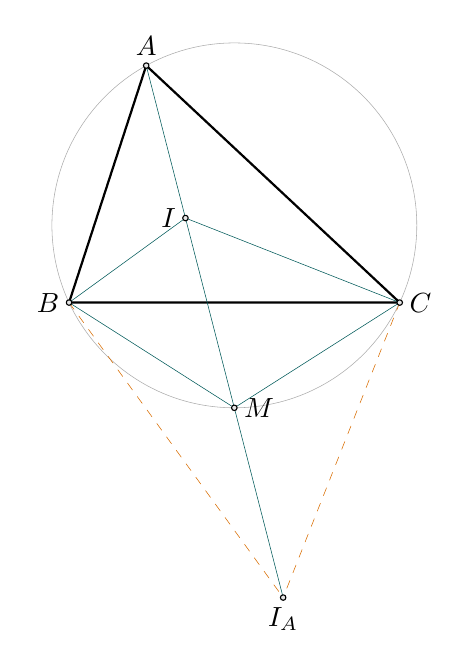
\begin{tikzpicture}[scale=.70]
\tkzDefPoints{0/0/B,6/0/C,1.4/4.3/A}
\tkzDefTriangleCenter[circum](A,B,C)\tkzGetPoint{O}
\tkzDefTriangleCenter[in](A,B,C)\tkzGetPoint{I}
\tkzInterLC[near](A,I)(O,A)\tkzGetPoints{Aagain}{M}
\tkzDefPointBy[symmetry=center M](I)\tkzGetPoint{IA}
\tkzDrawCircle[gray!65](O,A)
\tkzDrawPolygon[thick](A,B,C)
\tkzDrawSegments[teal!70!black](A,IA B,M C,M B,I C,I)
\tkzDrawSegments[dashed,orange!85!black](B,IA C,IA)
\tkzDrawPoints(A,B,C,I,M,IA)
\tkzLabelPoints[above](A)
\tkzLabelPoints[left](B,I)
\tkzLabelPoints[right](C)
\tkzLabelPoint[right](M){$M$}
\tkzLabelPoint[below](IA){$I_A$}
\end{tikzpicture}
\end{center}


\subsection{内心与外接圆联动时的操作顺序}
看到“内心加外接圆”，可先延长 $AI$ 至弧中点 $M$，把 $MI,MB,MC$ 统一成同一长度；看到内外角平分线同时出现，再考虑直径 $II_A$。这通常比直接列外角平分线比例更短。

\section{欧拉线 一次向量计算证明三个结论}
\level{提高：向量只用于解释结构，初中解题可改用中位线与相似}
以外心 $O$ 为原点，记顶点位置向量为 $\mathbf a,\mathbf b,\mathbf c$，它们的模长均为 $R$。定义 $\mathbf h=\mathbf a+\mathbf b+\mathbf c$，则
\[
 (\mathbf h-\mathbf a)\cdot(\mathbf b-\mathbf c)
 =(\mathbf b+\mathbf c)\cdot(\mathbf b-\mathbf c)=0.
\]
所以 $AH\perp BC$。循环置换，$H$ 同时落在三条高上，这也证明了垂心的存在。另一方面
\[
 \overrightarrow{OG}=\frac{\mathbf a+\mathbf b+\mathbf c}{3}
 =\frac13\overrightarrow{OH}.
\]
因此 $O,G,H$ 共线，且在非等边情形下 $OG:GH=1:2$，$G$ 在 $O,H$ 之间。这条线就是欧拉线。等边三角形中三点重合，不能由三个重合点定义唯一一条欧拉线。$I$ 一般不在欧拉线上，等腰三角形的对称轴是一个重要特例。

还可得到常用距离式
\[
 OH^2=9R^2-(a^2+b^2+c^2).
\]
这是因为 $\mathbf a\cdot\mathbf b=R^2-c^2/2$，将 $|\mathbf a+\mathbf b+\mathbf c|^2$ 展开即得。由定义推导，比记忆一串中心距离公式更稳定。

\section{九点圆的九个点为何在同一个圆上}
设 $N$ 为 $OH$ 的中点，即 $\mathbf n=\mathbf h/2$；设 $M_A$ 为 $BC$ 中点，$E_A$ 为 $AH$ 中点，则
\[
 \overrightarrow{NM_A}=-\frac{\mathbf a}{2},\qquad
 \overrightarrow{NE_A}=\frac{\mathbf a}{2}.
\]
所以 $M_A,E_A$ 是以 $N$ 为圆心、$R/2$ 为半径的圆上一对直径端点。循环可知三边中点和三条“顶点到垂心连线”的中点都在该圆上。

再设 $D_A$ 是 $A$ 到 $BC$ 的垂足。因为 $E_A,D_A$ 在高所在直线上，$M_A,D_A$ 在 $BC$ 上，故 $\angle E_AD_AM_A=90^\circ$，于是 $D_A$ 也在以 $E_AM_A$ 为直径的圆上。重合的特殊位置直接归入前述已知点。其他两个垂足同理。这就得到九点圆：三边中点、三垂足、三段 $AH,BH,CH$ 的中点；其圆心为 $OH$ 中点，半径为 $R/2$。名称“九点”不表示特殊三角形中这九点一定互异。可对照\href{https://gkfweb.math.illinois.edu/oldnew/math403/public/dilatations/dilatations.html}{Illinois 的相似变换证明}和\href{https://mathworld.wolfram.com/Nine-PointCircle.html}{九点圆资料}。

\section{欧拉公式 用鸡爪定理推导内外半径关系}
\begin{keybox}{欧拉公式及欧拉不等式}
任意非退化三角形都有
\[
 OI^2=R(R-2r),\qquad R\ge2r.
\]
等号 $R=2r$ 当且仅当三角形等边。
\end{keybox}
\begin{proof}
仍令 $M$ 为不含 $A$ 的弧 $BC$ 中点，令 $T$ 为 $I$ 到 $AB$ 的垂足。直角三角形 $AIT$ 中
$AI=r/\sin(A/2)$；外接圆弦长公式给出 $BM=2R\sin(A/2)$；鸡爪定理给出 $IM=BM$。于是
\[
 AI\cdot IM=2Rr.
\]
$I$ 位于圆内，直线 $AIM$ 上两割点位于 $I$ 两侧，因此圆幂为 $-AI\cdot IM$，得到 $OI^2-R^2=-2Rr$。
非负性给出 $R\ge2r$。等号等价于 $O=I$。若 $O=I$，圆心到三边距离相等，相应的三条弦等长，故 $a=b=c$；反之等边三角形显然满足等号。
\end{proof}
该公式的标准表述见\href{https://mathworld.wolfram.com/EulerTriangleFormula.html}{Euler Triangle Formula}。它是“圆周角、角平分线、圆幂”联动的结果，不宜作为没有来历的万能代入式。

\section{选读 旁心三角形与等角共轭}
\subsection{内心是旁心三角形的垂心}
$I_B,I_C$ 都在 $A$ 的外角平分线上，而 $A,I,I_A$ 在内角平分线上，故
\[
 II_A\perp I_BI_C.
\]
循环可得另两组垂直，所以 $I$ 是 $\triangle I_AI_BI_C$ 的垂心，$A,B,C$ 是它的三个垂足。旁心三角形的三个角分别为 $90^\circ-A/2$、$90^\circ-B/2$、$90^\circ-C/2$，因此它是锐角三角形。这里的“内心变垂心”建立在\textbf{换了参考三角形}这一点上。参阅\href{https://sites.math.washington.edu/~king/coursedir/m444a04/class/class29.html}{University of Washington 的旁心三角形课堂笔记}。

\subsection{等角共轭是把三条线同时反射}
对三角形内部一点 $P$，分别把 $AP,BP,CP$ 关于三个内角平分线反射，得到三条直线；它们仍共点于 $P^*$，称为 $P$ 的等角共轭。证明只需三角塞瓦：
\[
 \frac{\sin\angle BAP}{\sin\angle PAC}
 \frac{\sin\angle CBP}{\sin\angle PBA}
 \frac{\sin\angle ACP}{\sin\angle PCB}=1.
\]
它由普通塞瓦与下面的面积比公式及其循环式相乘得到：
\[
 \frac{BD}{DC}=\frac cb\frac{\sin\angle BAD}{\sin\angle DAC}.
\]
反射后每个正弦比倒置，乘积仍为 $1$，故三条反射线共点。此处内部条件保证我们讨论的是有限的内部交点；外部点的完整理论需加入有向角及无穷远情形。

内心 $I$ 的每条顶点连线就是反射轴，因此它是自身的等角共轭。在非直角三角形中，一个重要配对是外心 $O$ 与垂心 $H$：例如锐角情形下，$\angle BAH=90^\circ-B=\angle OAC$，所以 $AH,AO$ 关于 $A$ 的角平分线对称；另外两顶点同理。对钝角三角形应使用模 $180^\circ$ 的有向角处理直线方向。重心的等角共轭是对称中线点，不能把重心与垂心误配。定义及一般情形可查\href{https://mathworld.wolfram.com/IsogonalConjugate.html}{Isogonal Conjugate}。

\subsection{费尔巴哈定理放在什么位置}
\level{拓展事实：本讲义的两道试题不以此为前置结论}
非等边三角形的九点圆与内切圆内切，与三个旁切圆分别外切。若九点圆心为 $N$，对应的距离表述是
\[
 NI=\frac R2-r,\qquad NI_A=\frac R2+r_A
\]
及其循环式。\textbf{圆心距等于半径差或半径和}才是相切的证明目标，不能仅因图上接触就下结论。等边三角形中九点圆与内切圆重合，不能称为通常的唯一切点内切。这一完整定理的证明比本章的九点圆存在性深；后面的选读章将用向量和带符号的面积坐标给出完整证明，初学时可以先跳过。两道真题的解答不依赖费尔巴哈定理。参阅\href{https://mathworld.wolfram.com/FeuerbachsTheorem.html}{Feuerbach's Theorem}，以及给出完整向量证明的\href{https://arxiv.org/abs/1107.1152}{A Simple Vector Proof of Feuerbach's Theorem}。

\chapter{从共圆走向共线的两个模型}
\level{提高：每条辅助线都要说明服务于哪一个角}
\section{西姆松线 三个垂足的共线}
设 $P$ 在 $\triangle ABC$ 的外接圆上，向 $BC,CA,AB$ 所在直线作垂线，垂足依次为 $D,E,F$，则 $D,E,F$ 共线。这是西姆松定理\footnote{可查\href{https://mathworld.wolfram.com/SimsonLine.html}{Simson Line}。其逆定理也成立：三个垂足共线的点轨迹是三角形外接圆。}。
\begin{proof}
先处理各垂足互异、$P$ 不为顶点的一般情形。由直角可知 $P,D,E,C$ 共圆，$P,D,F,B$ 共圆。以下有向角均按模 $180^\circ$ 计算：
\begin{align*}
 \angle(DE,DF)
 &=\angle(DE,DP)+\angle(DP,DF)\\
 &=\angle(CE,CP)+\angle(BP,BF)\\
 &=\angle(CA,CP)+\angle(BP,BA)=0.
\end{align*}
最后一步使用了 $A,B,C,P$ 共圆，即 $\angle(CA,CP)=\angle(BA,BP)$。故 $DE,DF$ 是同一条直线。若垂足重合，则结论由其余两个点确定的直线直接成立；$P$ 为某顶点时，两垂足等于该顶点，第三垂足在对应高上，也共线。
\end{proof}
\textbf{识别信号：}一个圆上点，向三角形三边分别作垂线。实际压轴题可能只画了两个垂足，第三个是值得尝试的辅助点。不能见到三条垂线就套结论，$P$ 必须在外接圆上。

\section{米克尔点 用已知两圆找到第三圆}
设 $D,E,F$ 分别位于 $BC,CA,AB$ 所在直线，且不与对应顶点重合；相关三点均不共线。圆 $AEF$ 与圆 $BFD$ 除 $F$ 外另交于 $P$，则 $P$ 也在圆 $CDE$ 上。
\begin{proof}
若 $P$ 与 $C,D,E$ 中某点重合，结论显然；以下设这四点互异。按模 $180^\circ$ 计算，有
\begin{align*}
 \angle(PD,PE)
 &=\angle(PD,PF)+\angle(PF,PE)\\
 &=\angle(BD,BF)+\angle(AF,AE)\\
 &=\angle(BC,BA)+\angle(AB,AC)\\
 &=\angle(BC,AC)=\angle(CD,CE).
\end{align*}
所以 $P,D,E,C$ 共圆。证明中只用了圆周角与角的可加性。
\end{proof}
这里明确假设两圆存在不同于 $F$ 的第二交点；相切或三点共线的退化情形需要另行处理，不应在图形不存在时生搬定理。标准三角形及四直线版本见\href{https://mathworld.wolfram.com/MiquelsTheorem.html}{Miquel's Theorem}。


\chapter{五心的补充工具 面积切点与垂足}
\level{核心补充：把中心定义转成具体可用的面积和长度}
\section{重心 面积等分与平方和最小}
设 $D,E,F$ 分别为 $BC,CA,AB$ 的中点，三中线交于重心 $G$。
中线把三角形分成两个等面积三角形；从 $G$ 到同一条边的两个小三角形也同高，所以
\[
 [GBD]=[GCD],\quad [GCE]=[GAE],\quad [GAF]=[GBF].
\]
又因 $AG:GD=2:1$，同底 $BD$ 的三角形 $ABD,GBD$ 面积比为 $3:1$，而 $[ABD]=\Delta/2$，故 $[GBD]=\Delta/6$。循环可知\textbf{三中线分出的六个小三角形等面积}，从而
\[
 [GAB]=[GBC]=[GCA]=\frac{\Delta}{3}.
\]
反过来，若内部点 $P$ 满足上述三个大块面积相等，则其到 $BC,CA,AB$ 的有向面积坐标均为 $1/3$，所以 $P=G$。若不使用面积坐标，令 $Q=AP\cap BC$。由同高及共同的顶点到直线 $AP$ 的距离关系，有 $[PAB]/[PAC]=BQ/QC=1$，故 $Q=D$；再结合 $[PBC]=\Delta/3$ 得 $AP:PD=2:1$，从而确定重心。

对平面内任一点 $P$，还有
\[
 PA^2+PB^2+PC^2=3PG^2+\frac{a^2+b^2+c^2}{3}.
\]
\begin{proof}
以 $G$ 为原点，记顶点向量为 $\mathbf u,\mathbf v,\mathbf w$，则 $\mathbf u+\mathbf v+\mathbf w=0$。把三个平方展开，交叉项之和为零，得到
$PA^2+PB^2+PC^2=3PG^2+GA^2+GB^2+GC^2$。
再展开 $|\mathbf u-\mathbf v|^2+|\mathbf v-\mathbf w|^2+|\mathbf w-\mathbf u|^2$，利用向量和为零，得到 $a^2+b^2+c^2=3(GA^2+GB^2+GC^2)$，代入即得。
\end{proof}
因此距离平方和在 $P=G$ 时取得唯一最小值 $(a^2+b^2+c^2)/3$。这里最小化的是\emph{平方和}，不是距离和；三条距离之和的最小点一般不是重心。

\section{垂心的反射 为什么值得补一个对称点}
若 $\triangle ABC$ 为锐角三角形，垂心为 $H$，$H'$ 为 $H$ 关于 $BC$ 的对称点，则 $H'$ 在外接圆上。
\begin{proof}
由于 $BH\perp AC$、$CH\perp AB$，锐角情形下 $\angle BHC=180^\circ-A$。反射保持角度，故 $\angle BH'C=180^\circ-A$。$A,H'$ 位于 $BC$ 两侧，两角互补，于是 $A,B,H',C$ 共圆。钝角情形可用同一事实的有向角版本：反射将 $\angle(HB,HC)$ 变号，而两组垂直把该角转成顶点 $A$ 的负角，故结论依旧成立。直角三角形中，对称点可能与原顶点重合，应单独理解。
\end{proof}
另外，$H$ 关于 $BC$ 中点的对称点 $H''$ 也在外接圆上。因为 $BH''\parallel CH\perp AB$，$CH''\parallel BH\perp AC$，所以 $\angle ABH''=\angle ACH''=90^\circ$，圆 $ABCH''$ 以 $AH''$ 为直径。若辅助图需要一条直径或一组平行，这个中点对称往往比轴对称更合适。

\section{锐角三角形的垂足三角形 垂心变内心}
设 $D,E,F$ 分别是锐角三角形 $ABC$ 的三个垂足，即 $D\in BC,E\in CA,F\in AB$。则 $H$ 是 $\triangle DEF$ 的内心。
\begin{proof}
由直角得 $C,D,H,E$ 共圆，$B,D,H,F$ 共圆。于是
\[
 \angle EDH=\angle ECH=90^\circ-A,
 \qquad
 \angle HDF=\angle HBF=90^\circ-A.
\]
这些角为正，且对应于 $\angle EDF$ 内部的两部分，因此 $DH$ 平分 $\angle EDF$。循环得到 $EH,FH$ 平分另外两个内角，所以 $H$ 是垂足三角形的内心。还可读出垂足三角形的三个角为 $180^\circ-2A,180^\circ-2B,180^\circ-2C$。
\end{proof}
\begin{center}
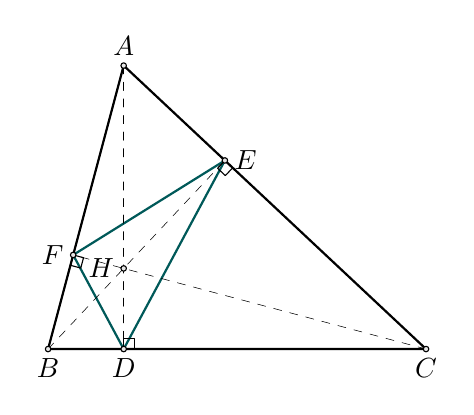
\begin{tikzpicture}[scale=.80]
\tkzDefPoints{0/0/B,6/0/C,1.2/4.5/A}
\tkzDefPointBy[projection=onto B--C](A)\tkzGetPoint{D}
\tkzDefPointBy[projection=onto C--A](B)\tkzGetPoint{E}
\tkzDefPointBy[projection=onto A--B](C)\tkzGetPoint{F}
\tkzInterLL(A,D)(B,E)\tkzGetPoint{H}
\tkzDrawPolygon[thick](A,B,C)
\tkzDrawPolygon[thick,teal!70!black](D,E,F)
\tkzDrawSegments[dashed](A,D B,E C,F)
\tkzMarkRightAngles[size=.17](A,D,C B,E,C C,F,B)
\tkzDrawPoints(A,B,C,D,E,F,H)
\tkzLabelPoints[above](A)
\tkzLabelPoints[below](B,C,D)
\tkzLabelPoints[right](E)
\tkzLabelPoints[left](F,H)
\end{tikzpicture}
\end{center}
锐角条件不能省掉。钝角三角形的垂心在原三角形外部，相应角平分线的内外关系改变；不能未经位置分析就继续称它为垂足三角形的内心。

\section{欧拉线与九点圆的图形总览}
\begin{center}
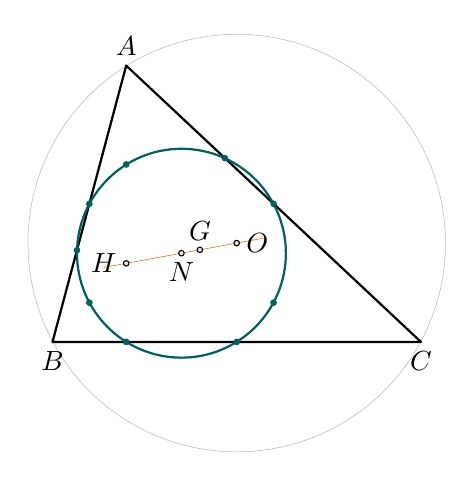
\begin{tikzpicture}[scale=.78]
\tkzDefPoints{0/0/B,6/0/C,1.2/4.5/A}
\tkzDefTriangleCenter[circum](A,B,C)\tkzGetPoint{O}
\tkzDefTriangleCenter[ortho](A,B,C)\tkzGetPoint{H}
\tkzDefTriangleCenter[centroid](A,B,C)\tkzGetPoint{G}
\tkzDefMidPoint(O,H)\tkzGetPoint{N}
\tkzDefMidPoint(B,C)\tkzGetPoint{D}
\tkzDefMidPoint(C,A)\tkzGetPoint{E}
\tkzDefMidPoint(A,B)\tkzGetPoint{F}
\tkzDefMidPoint(A,H)\tkzGetPoint{U}
\tkzDefMidPoint(B,H)\tkzGetPoint{V}
\tkzDefMidPoint(C,H)\tkzGetPoint{W}
\tkzDefPointBy[projection=onto B--C](A)\tkzGetPoint{Da}
\tkzDefPointBy[projection=onto C--A](B)\tkzGetPoint{Ea}
\tkzDefPointBy[projection=onto A--B](C)\tkzGetPoint{Fa}
\tkzDrawCircle[gray!55](O,A)
\tkzDrawPolygon[thick](A,B,C)
\tkzDrawCircle[teal!75!black,thick](N,D)
\tkzDrawLine[add=.20 and .25,orange!85!black](H,O)
\tkzDrawPoints[size=2,teal!75!black](D,E,F,U,V,W,Da,Ea,Fa)
\tkzDrawPoints(H,N,G,O)
\tkzLabelPoints[above](A,G)
\tkzLabelPoints[below](B,C,N)
\tkzLabelPoints[left](H)
\tkzLabelPoints[right](O)
\end{tikzpicture}
\end{center}
青色圆上标出了九个构造点；橙色线为 $H,N,G,O$ 所在的欧拉线。图中的字母顺序是沿线的实际顺序 $H,N,G,O$，且 $HN:NO=1:1$、$HG:GO=2:1$。若特殊三角形造成点重合，按前文相应条件处理。图中没有把内心放到欧拉线上，因为一般并不成立。

\section{切线长把半周长变成几何线段}
设内切圆分别切 $BC,CA,AB$ 于 $D,E,F$。同一点引圆的两条切线等长，令
$AF=AE=x$、$BF=BD=y$、$CD=CE=z$，则
\[
 x+y=c,\qquad y+z=a,\qquad z+x=b.
\]
相加得 $x+y+z=s$，所以
\[
 AF=AE=s-a,\quad BD=BF=s-b,\quad CE=CD=s-c.
\]
这些是把“周长条件”转成“切点线段”的桥梁，不要把 $BD$ 误记成 $s-a$。

\subsection{一个塞瓦小例 热尔岗点}
由上述切线长立即得到
\[
 \frac{BD}{DC}\frac{CE}{EA}\frac{AF}{FB}
 =\frac{s-b}{s-c}\frac{s-c}{s-a}\frac{s-a}{s-b}=1.
\]
所以 $AD,BE,CF$ 共点。该点称为热尔岗点（Gergonne point），一般既不是重心，也不是内心。这里没有引入新的证明技术：是三个切线长等式经过塞瓦合在一起。名称参见\href{https://mathworld.wolfram.com/GergonnePoint.html}{Gergonne Point}。

\subsection{旁切圆切点与奈格尔点}
$A$ 旁切圆切 $BC$ 于 $D_A$，则
\[
 BD_A=s-c,\qquad D_AC=s-b.
\]
为验证位置和次序，令它与射线 $AB,AC$ 越过 $B,C$ 后的切点为 $F_A,E_A$。同点切线长给出 $AF_A=AE_A$、$BF_A=BD_A=x$、$CE_A=CD_A=y$，于是 $c+x=b+y$、$x+y=a$，解得 $x=s-c,y=s-b$。另外两边的旁切点循环定义，有
\[
 \frac{BD_A}{D_AC}\frac{CE_B}{E_BA}\frac{AF_C}{F_CB}
 =\frac{s-c}{s-b}\frac{s-a}{s-c}\frac{s-b}{s-a}=1.
\]
故 $AD_A,BE_B,CF_C$ 共点，称奈格尔点（\href{https://mathworld.wolfram.com/NagelPoint.html}{Nagel point}）。内切点和相应旁切点在同一条边上的两段长度次序互换，正是两个塞瓦乘积都能约去的原因。

\chapter{辅助线为什么这样添}
\section{先确定要搬运的对象}
旋转保持长度、角度、共线和图形的方向。绕 $O$ 旋转同一个有向角 $\theta$，若 $A\mapsto B$、$C\mapsto D$，则线段 $AC$ 也映为 $BD$，所以 $AC=BD$；两条承载直线的夹角为 $\theta$ 模 $180^\circ$。当 $\theta=90^\circ$ 且线段非零时，还得到 $AC\perp BD$。

\begin{keybox}{旋转的四个要素}
必须同时说清旋转中心、旋转方向与角度、对应点、构造目的。只看见等腰三角形并不足以启动旋转。尝试把一条已知等长边送到另一条边，再检查另一端点的像是否落在有用的线、圆或交点上。
\end{keybox}
\section{手拉手模型与方向检查}
设 $OAB$、$OCD$ 是两个顶点按相同方向排列的等边三角形。绕 $O$ 逆时针旋转 $60^\circ$，有 $A\mapsto B$、$C\mapsto D$，故 $AC=BD$。若两等边三角形的排列方向相反，则这个对应不成立，应重新选择对应点；不能只凭“都有 $60^\circ$”就判全等。
\begin{center}
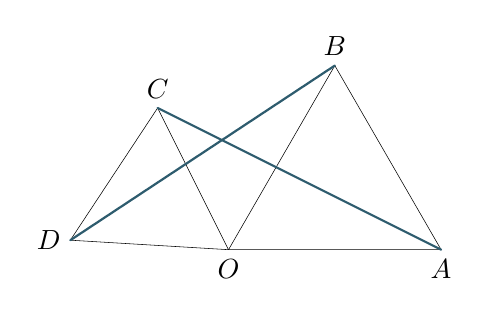
\begin{tikzpicture}[scale=.9]
\tkzDefPoints{0/0/O,3/0/A,-1/2/C}
\tkzDefPointBy[rotation=center O angle 60](A)\tkzGetPoint{B}
\tkzDefPointBy[rotation=center O angle 60](C)\tkzGetPoint{D}
\tkzDrawPolygon(O,A,B)\tkzDrawPolygon(O,C,D)
\tkzDrawSegments[hint](A,C B,D)
\tkzLabelPoints[below](O,A)\tkzLabelPoints[above](B,C)\tkzLabelPoints[left](D)
\end{tikzpicture}
\figcaption{同向的两组旋转使两条分散的线段成为对应边。}
\end{center}
\level{迁移}把 $60^\circ$ 换成 $90^\circ$，把两个等边三角形换成公共顶点处的两组等长垂直线段，便得到“等长且垂直”的模型。长度相等只给出一组距离条件；必须再核对同向夹角才能使用同一次旋转。
\section{一道真正需要拼接长度的例题}
\level{例题}在等边三角形 $ABC$ 内取点 $P$，满足 $\angle APB=150^\circ$。证明 $PA^2+PB^2=PC^2$。

\level{为什么想到旋转}目标是平方和，盼望出现一条以 $PA,PB$ 为直角边、以 $PC$ 为斜边的直角三角形。原图的 $150^\circ$ 距离直角恰好差 $60^\circ$，等边三角形恰好能提供这一旋转角。

\level{构造与证明}将三角形 $BAP$ 绕 $B$ 顺时针旋转 $60^\circ$（图中 $A\mapsto C$），设 $P\mapsto P'$。由旋转，$CP'=AP$，$BP'=BP$，且 $\angle PBP'=60^\circ$，所以 $BPP'$ 等边，$PP'=BP$。又 $\angle BP'C=\angle BPA=150^\circ$，$\angle BP'P=60^\circ$；因 $P$ 为内部点，射线 $BC$ 位于 $\angle PBP'$ 内部，$C,P$ 在直线 $BP'$ 同侧，故射线 $P'P$ 位于该 $150^\circ$ 角内，故 $\angle PP'C=90^\circ$。在直角三角形 $PP'C$ 中，
\[
 PC^2=PP'^2+P'C^2=PB^2+PA^2.
\]
\begin{center}
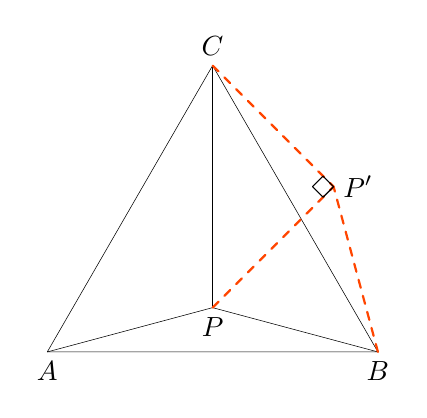
\begin{tikzpicture}[scale=1.05]
\tkzDefPoints{0/0/A,4/0/B,2/3.4641016/C,2/.5358984/P}
\tkzDefPointBy[rotation=center B angle -60](P)\tkzGetPoint{PP}
\tkzDrawPolygon(A,B,C)\tkzDrawSegments(A,P B,P C,P)
\tkzDrawSegments[aux](P,PP B,PP C,PP)
\tkzMarkRightAngle[size=.18](P,PP,C)
\tkzLabelPoints[below](A,B,P)\tkzLabelPoints[above](C)
\tkzLabelPoint[right](PP){$P'$}
\end{tikzpicture}
\figcaption{把 $PA$ 搬到 $P'C$，同时让 $PB$ 成为 $PP'$，终于进入同一个直角三角形。}
\end{center}
\level{角序如何复核}上述顺时针方向由图中 $A\mapsto C$ 唯一确定。若把三角形翻到另一侧，则相应改为逆时针，不能沿用同一角序。证明中的 $150^\circ-60^\circ$ 必须明确是哪两条射线之间的差。
\section{与其他辅助线的选择比较}
\begin{center}\small
\begin{tabular}{p{.25\linewidth}p{.28\linewidth}p{.32\linewidth}}
\toprule
条件信号&优先候选&希望新增的联系\\\midrule
等长且有同向定角&旋转&两组对应边、长度拼接\\
角平分线、到直线等距&翻折或作垂线&两直角三角形全等\\
中点、中线与倍数&倍长中线、中位线&平行四边形、重心\\
两个相等角、边的比&相似或作平行线&比例方程\\
平方和与直径&作高、连接直径端点&直角、勾股定理\\
两条相交等弦&圆心到弦的垂线&等弦等距、全等\\\bottomrule
\end{tabular}\end{center}
上海题恰好属于最后一种信号。等弦使圆心到两弦的距离相等；从圆心作垂线后即可判全等，没有必要强行旋转。浙江题中的 $AC=AD$ 先提供等腰三角形，再由直角与圆周角逐层追踪。

\begin{keybox}{做完一道题后的四行笔记}
原目标缺少什么关系？题中哪个条件最早暗示构造？新增线段属于哪个三角形或哪个圆？把辅助线去掉后，是否还能从原条件重新想到它？能回答这四行，才算把一次解答变成可迁移的方法。
\end{keybox}

% 本片段只定义本讲义所用图形，不改动 beautybook 类或任何模板样式。
\newcommand{\SHpoints}{%
  \tkzDefPoints{-2.0615528128088/0.0000000000000/A,-0.3638034375545/1.4552137502180/P,1.8190171877725/0.9701425001453/C,0.8488746876272/0.7276068751090/E,2.0615528128088/0.0000000000000/Q,0.0000000000000/0.0000000000000/O,-0.1212678125182/0.4850712500727/K,-1.7220029377580/0.2910427500436/F,0.3152963125472/2.0372992503052/B,-1.2369316876853/1.6492422502471/D}%
}
\newcommand{\SHcalcpoints}{%
  \tkzDefPoints{0.0000000000000/0.0000000000000/O,-2.0000000000000/0.0000000000000/A,2.0000000000000/0.0000000000000/Q,-0.1093750000000/1.9970070378882/B,-0.7968750000000/1.2708226604743/P,-0.0820312500000/1.4977552784161/H,0.8710937500000/1.8003321023386/C,-1.7500000000000/0.9682458365519/D}%
}
\newcommand{\SHoutline}{%
  \tkzDrawArc[thick](O,Q)(A)
  \tkzDrawSegments(A,Q A,B C,D)
  \tkzDrawPoints[size=2](O,P)
  \tkzLabelPoints[below left](A)
  \tkzLabelPoints[below right](Q)
  \tkzLabelPoints[below](O)
  \tkzLabelPoints[above](B)
  \tkzLabelPoints[above left](D)
  \tkzLabelPoints[right](C)
  \tkzLabelPoints[above left](P)
}
\newcommand{\SHproblemfig}[1]{%
  \begin{tikzpicture}[scale=.88]
  \ifnum#1=2\SHcalcpoints\else\SHpoints\fi\SHoutline
  \ifnum#1=1\tkzDrawSegments(O,P)\fi
  \ifnum#1=2
    \tkzInterLL(O,B)(C,D)\tkzGetPoint{H}%
    \tkzDrawSegments(O,B O,P)\tkzLabelPoints[above right](H)
  \fi
  \ifnum#1=3
    \tkzDrawSegments(P,Q A,C F,Q)\tkzLabelPoints[below](E)
    \tkzLabelPoints[left](F)
  \fi
  \end{tikzpicture}}
\newcommand{\ZJpoints}[1]{%
  \tkzDefPoints{-1/0/A,1/0/B,0/0/O}%
  \ifnum#1=1
    \tkzDefPoints{-.8090169944/.5877852523/C,-.3819660113/0/D,.3090169944/-.9510565163/E,-.1180339887/.3632712640/F,-.6180339887/0/G,-.4635254916/.1122569941/H}%
  \fi
  \ifnum#1=2
    \tkzDefPoints{-.6427876097/.7660444431/C,-.1547634765/0/D,.4226182617/-.9063077870/E,.0260823620/.4541452530/F,-.6867828916/0/G,-.3083526239/.2410866694/H}%
  \fi
  \ifnum#1=3
    \tkzDefPoints{-.0979797464/.9951884089/C,.3431457505/0/D,.6715728753/-.7409385084/E,.3994949366/.5442866141/F,-.8284271247/0/G,.1507575951/.4340317293/H}%
  \fi}
\newcommand{\ZJoutline}{%
  \tkzDrawCircle[thick](O,A)
  \tkzDrawSegments(A,B A,C C,B C,E B,E F,G)
  \tkzMarkRightAngle[size=.07](C,H,F)
  \tkzDrawPoints[size=1.5](O,D,G,H,F)
  \tkzLabelPoints[left](A)
  \tkzLabelPoints[right](B)
  \tkzLabelPoints[above](C)
  \tkzLabelPoints[below right](E)
  \tkzLabelPoints[below](O,G)
  \tkzLabelPoints[above right](D,F)
  \tkzLabelPoints[above left](H)
}

\chapter{上海压轴题 从等弦走向重心}
\level{学习目标}把等弦、到两边距离相等、角平分线、等腰三角形和重心连接成一条可重复使用的推理链。

\section{原题重排与图形阅读}
在半圆 $AOQ$ 中，点 $O$ 为圆心，线段 $AQ$ 为直径，$B$、$C$ 是半圆上两点，$D$ 是弧 $AB$ 上一点，连接 $AB$、$CD$ 交于点 $P$，且 $AB=CD$。\footnote{用户提供的 Word 正文中“$D$ 是 $AB$ 上一点”缺弧符号；根据原题三图补作“弧 $AB$”。若理解为直线 $AB$，则两条连线交点成为 $D$，与原图及后续条件不符。}

（1）如图1，连接 $OP$。
\begin{enumerate}[label=\textcircled{\scriptsize\arabic*},leftmargin=2em]
\item 求证：$\angle APO=\angle CPO$。
\item 如图2，连接 $OB$ 交弦 $CD$ 于点 $H$。若 $AQ=4$，$PB=1$，$PO=HO$，求 $PH$ 的长。
\end{enumerate}
（2）如图3，连接 $PQ$、$AC$ 交于点 $E$。线段 $AP$ 上有一点 $F$，使得 $PF=4AF$。若 $PE=QE$，$\angle PEA=\angle PFQ$，求 $\frac{PE}{EA}$ 的值。

\begin{center}
\begin{minipage}[t]{.32\linewidth}\centering\SHproblemfig{1}\figcaption{图1 等弦与角平分线}\end{minipage}\hfill
\begin{minipage}[t]{.32\linewidth}\centering\SHproblemfig{2}\figcaption{图2 $H=OB\cap CD$}\end{minipage}\hfill
\begin{minipage}[t]{.32\linewidth}\centering\SHproblemfig{3}\figcaption{图3 $E=PQ\cap AC$}\end{minipage}
\end{center}
\level{先读结构}图1的关键是两条相等的弦；图2把角平分线结论放入等腰三角形；图3增加了两个中点信号：$O$ 是 $AQ$ 的中点，$E$ 是 $PQ$ 的中点。

\section{第一问 用到两边的距离证明平分角}
\subsection{为什么要从圆心向弦作垂线}
所求是 $\angle APO=\angle CPO$，也就是 $PO$ 平分 $\angle APC$。角平分线上的点到两边距离相等，因此可以反过来寻找圆心 $O$ 到 $PA$、$PC$ 的两段垂线。等弦恰好能提供相等的弦心距。

\begin{center}
\begin{tikzpicture}[scale=1.15]
\SHpoints\SHoutline
\tkzDefPointBy[projection=onto A--B](O)\tkzGetPoint{G}
\tkzDefPointBy[projection=onto C--D](O)\tkzGetPoint{Z}
\tkzDrawSegments(O,P)
\tkzDrawSegments[aux](O,G O,Z O,C)
\tkzMarkRightAngle[size=.12](O,G,A)
\tkzMarkRightAngle[size=.12](O,Z,C)
\tkzLabelPoints[below left](G)
\tkzLabelPoints[above right](Z)
\end{tikzpicture}
\figcaption{图4 两次 HL 全等：先得 $OG=OZ$，再得 $\angle APO=\angle CPO$。}
\end{center}

\level{完整证明}作 $OG\perp AB$ 于 $G$，$OZ\perp CD$ 于 $Z$，连接 $OC$。由垂径定理，
\[
 AG=\frac12AB,\qquad CZ=\frac12CD.
\]
因 $AB=CD$，所以 $AG=CZ$。又 $OA=OC$，故
\[
 \mathrm{Rt}\triangle OAG\cong\mathrm{Rt}\triangle OCZ\quad(\mathrm{HL}),
\]
从而 $OG=OZ$。在直角三角形 $OPG$ 与 $OPZ$ 中，$OP$ 是公共斜边，$OG=OZ$，所以
\[
 \mathrm{Rt}\triangle OPG\cong\mathrm{Rt}\triangle OPZ\quad(\mathrm{HL}).
\]
于是 $\angle GPO=\angle ZPO$。由原图 $A,G,P,B$ 依次共线、$D,P,Z,C$ 依次共线，得到
\[
 \boxed{\angle APO=\angle CPO}.
\]

\begin{keybox}{把中间结论留下来}
第二次全等还给出 $PG=PZ$。结合 $AG=CZ$，得到
\[
 AP=AG+GP=CZ+ZP=CP.
\]
所以 $\triangle APC$ 是等腰三角形。$PO$ 是顶角平分线，因此也是底边 $AC$ 的垂直平分线。后面要用的并不只是一个角相等，而是
\[
 \boxed{PA=PC,\qquad PO\perp AC,\qquad PO\text{ 平分 }AC.}
\]
这里仅使用角平分线和等腰三角形的基本性质，无需外角平分线定理。
\end{keybox}

\section{第一问的计算 把等腰转成相似}
\begin{center}
\begin{tikzpicture}[scale=1.18]
\SHcalcpoints\SHoutline
\tkzDrawSegments(O,B O,P)
\tkzDrawSegments[aux](B,P P,H)
\tkzLabelPoints[above right](H)
\end{tikzpicture}
\figcaption{图5 $PO=HO$ 提供等角，$B,P,A$ 与 $B,H,O$ 的共线关系负责转角。}
\end{center}

\level{第一步 从等腰取角}由 $PO=HO$，得
\[
 \angle OPH=\angle OHP.
\]
由第一问，$\angle OPH=\angle APO$，因此 $\angle APO=\angle OHP$。
又 $PA$ 与 $PB$ 反向，$HO$ 与 $HB$ 反向，所以
\[
 \angle BPO=180^\circ-\angle APO
 =180^\circ-\angle OHP=\angle BHP.
\]

\level{第二步 按对应顺序写相似}$\angle PBH=\angle OBP$，故
\[
 \triangle BPH\sim\triangle BOP,
 \qquad
 \frac{BP}{BO}=\frac{BH}{BP}=\frac{PH}{OP}.
\]
对应关系是 $B\leftrightarrow B$，$P\leftrightarrow O$，$H\leftrightarrow P$；写比例前先核对这一点。

\level{第三步 用线段和求长度}由 $AQ=4$，得 $BO=2$；又 $BP=1$，所以
\[
 BH=\frac{BP^2}{BO}=\frac12,\qquad PH=\frac12OP.
\]
由于 $B,H,O$ 依次共线，
\[
 OH=OB-BH=2-\frac12=\frac32.
\]
再由 $OP=OH$，得
\[
 \boxed{PH=\frac12\cdot\frac32=\frac34}.
\]

\section{第二问 相似给比例 重心给位置}
\subsection{先解决长度之间的乘积关系}
\level{从等角识别相似}已知 $\angle PFQ=\angle PEA$。又 $P,F,A$ 共线，$P,E,Q$ 共线，因此
\[
 \angle FPQ=\angle EPA.
\]
于是
\[
 \triangle FPQ\sim\triangle EPA,
 \qquad \frac{PF}{PE}=\frac{PQ}{PA}.
\]
设 $AF=m>0$，$PE=QE=n>0$。则
\[
 PF=4m,\qquad PA=5m,\qquad PQ=2n.
\]
代入比例，得
\[
 \frac{4m}{n}=\frac{2n}{5m}
 \quad\Longrightarrow\quad n^2=10m^2
 \quad\Longrightarrow\quad \boxed{PE=\sqrt{10}\,m}.
\]
这一步还没有求出 $EA$，所以不能在这里停下来。

\subsection{为什么在这里想到重心}
\begin{center}
\begin{tikzpicture}[scale=1.18]
\SHpoints\SHoutline
\tkzDrawSegments(P,Q A,C F,Q)
\tkzDrawSegments[aux](P,O)
\tkzLabelPoints[below](E)
\tkzLabelPoints[left](F)
\tkzLabelPoints[below left](K)
\tkzMarkRightAngle[size=.12](P,K,A)
\end{tikzpicture}
\figcaption{图6 在 $\triangle APQ$ 中看两条中线：$PO$ 与 $AE$ 交于重心 $K$。}
\end{center}

连接 $PO$，交 $AC$ 于 $K$。由第一问保留的结论，$PA=PC$，且 $PO\perp AC$。
在 $\triangle APQ$ 中，$O$ 是 $AQ$ 的中点，$E$ 是 $PQ$ 的中点；$PO$ 与 $AE$ 都是中线，它们的交点 $K$ 是重心。所以
\[
 \boxed{AK=2KE}.
\]
这里的 $2:1$ 是同一条中线上“顶点到重心”和“重心到对边中点”的比，不能把 $P$、$A$、$E$ 的位置混用。

\subsection{用同一条直角边消元}
设 $EK=k>0$，则 $AK=2k$，$EA=3k$。
在直角三角形 $APK$ 与 $EPK$ 中，共同的直角边 $PK$ 给出
\[
 PK^2=AP^2-AK^2=PE^2-EK^2.
\]
代入 $AP=5m$、$PE=\sqrt{10}\,m$，得
\[
 (5m)^2-(2k)^2=(\sqrt{10}\,m)^2-k^2,
 \qquad 3k^2=15m^2.
\]
故 $k=\sqrt5\,m$，从而
\[
 \boxed{\frac{PE}{EA}=\frac{\sqrt{10}\,m}{3\sqrt5\,m}
 =\frac{\sqrt2}{3}}.
\]

\begin{keybox}{整题的迁移路线}
等弦 $\Rightarrow$ 弦心距相等 $\Rightarrow$ 角平分线；保留全等中的线段相等，得到 $PA=PC$；两个中点 $\Rightarrow$ 两条中线 $\Rightarrow$ 重心；最后把同一条直角边写成两个勾股式。图中出现一个圆，并不意味着最后一步仍要使用圆的定理。
\end{keybox}

\chapter{浙江压轴题 从角度参数走向共线}
\level{学习目标}先用 $\alpha$ 管理角度，再把长度条件转成全等或相似；遇到共线结论，明确说明射线的位置。

\section{原题重排与三种位置}
如图1，$\triangle ABC$ 内接于 $\odot O$，$D$ 是直径 $AB$ 上的一点，满足 $AC=AD$。连接 $CD$ 并延长交 $\odot O$ 于点 $E$，连接 $BE$。点 $F$ 在弦 $BC$ 上，且 $BF=DE$。过点 $F$ 作 $FG\perp CE$，交 $AB$ 于点 $G$，交 $CD$ 于点 $H$。设 $\angle CAB=\alpha$。

（1）用含 $\alpha$ 的代数式表示 $\angle ABE$ 和 $\angle FGB$ 的大小。

（2）如图1，若 $CF=CD$，求证：$GF=GO$。

（3）如图3，若 $\odot O$ 的半径为 $1$，点 $D$ 在 $OB$ 上，且 $OD=2AG$，求 $AC$ 的长。

\begin{center}
\begin{minipage}[t]{.32\linewidth}\centering
\begin{tikzpicture}[scale=1.55]\ZJpoints{1}\ZJoutline\end{tikzpicture}
\figcaption{图1 $D$ 在 $AO$ 上}\end{minipage}\hfill
\begin{minipage}[t]{.32\linewidth}\centering
\begin{tikzpicture}[scale=1.55]\ZJpoints{2}\ZJoutline\end{tikzpicture}
\figcaption{图2 同一构造的另一位置}\end{minipage}\hfill
\begin{minipage}[t]{.32\linewidth}\centering
\begin{tikzpicture}[scale=1.55]\ZJpoints{3}\ZJoutline\end{tikzpicture}
\figcaption{图3 $D$ 在 $OB$ 上}\end{minipage}
\end{center}
\level{读图时特别留意}$D$、$O$ 的左右顺序在前两图与图3不同。涉及 $OD$、$BD$ 的线段加减时，必须重新核对图3，不能沿用图1的位置。

\section{第一问 先建立统一的角度表}
由 $AC=AD$，$\angle CAD=\alpha$，得
\[
 \angle ACD=\angle ADC
 =\frac{180^\circ-\alpha}{2}=90^\circ-\frac\alpha2.
\]
$\angle ABE$ 与 $\angle ACE$ 同对弧 $AE$，且 $C,D,E$ 依次共线，因此
\[
 \boxed{\angle ABE=\angle ACE=90^\circ-\frac\alpha2}.
\]
又 $FG\perp CE$，$D,G,B$ 共线，所以
\[
 \boxed{\angle FGB=90^\circ-\angle ADC=\frac\alpha2}.
\]
\begin{keybox}{先存好四个角}
\[
\begin{aligned}
\angle ACD=\angle ADC&=90^\circ-\frac\alpha2,\\
\angle ABE&=90^\circ-\frac\alpha2,\\
\angle FGB&=\frac\alpha2,\\
\angle ABC&=90^\circ-\alpha.
\end{aligned}
\]
最后一式来自直径所对圆周角 $\angle ACB=90^\circ$。后两问都可以直接调用这些角。
\end{keybox}

\section{第二问 用全等找到共线的桥梁}
\subsection{从线段和得到特殊角 $72^\circ$}
$\angle CEB$ 与 $\angle CAB$ 同对弧 $CB$，所以 $\angle CEB=\alpha$。
又
\[
 \angle CBE=\angle ABC+\angle ABE
 =(90^\circ-\alpha)+(90^\circ-\tfrac\alpha2)
 =180^\circ-\frac{3\alpha}{2}.
\]
由 $CF=CD$、$BF=DE$，得到
\[
 CB=CF+FB=CD+DE=CE.
\]
于是 $\triangle CBE$ 等腰，$\angle CBE=\angle CEB$，故
\[
 \alpha=180^\circ-\frac{3\alpha}{2},\qquad
 \boxed{\alpha=72^\circ}.
\]
从而
\[
 \angle CEB=\angle CBE=72^\circ,\quad
 \angle BCE=36^\circ,\quad \angle FGB=36^\circ.
\]

\subsection{构造全等 把一个角搬到圆心}
\begin{center}
\begin{tikzpicture}[scale=2.25]
\ZJpoints{1}\ZJoutline
\tkzDrawSegments[aux](O,F O,E)
\end{tikzpicture}
\figcaption{图7 连接 $OF$、$OE$：$\triangle OED\cong\triangle OBF$ 把角移到 $O$。}
\end{center}

连接 $OF$、$OE$。由圆心角定理，
\[
 \angle BOE=2\angle BCE=72^\circ.
\]
$OB=OE$，故 $\angle OBE=\angle OEB=54^\circ$。
于是
\[
 \angle OED=\angle CEB-\angle OEB=18^\circ,
 \qquad \angle OBF=\angle ABC=18^\circ.
\]
在 $\triangle OED$ 与 $\triangle OBF$ 中，$OE=OB$、$ED=BF$，且两边的夹角 $\angle OED=\angle OBF$，所以
\[
 \triangle OED\cong\triangle OBF\quad(\mathrm{SAS}).
\]
由对应角相等，得 $\angle DOE=\angle BOF$。

\subsection{说明射线位置 再使用补角}
由直角三角形 $ABC$，$AD=AC=AB\cos72^\circ<AB/2=AO$，故 $D$ 在 $AO$ 上。于是 $D,O,B$ 依次共线，所以
\[
 \angle DOE+\angle BOE=180^\circ.
\]
故 $\angle BOF+\angle BOE=180^\circ$。又 $F$ 与 $E$ 分别在 $AB$ 的两侧，$OF$ 与 $OE$ 位于 $OB$ 的两侧，因此 $OF$ 与 $OE$ 是反向射线，即
\[
 \boxed{F,O,E\text{ 三点共线}}.
\]
不能仅看到两个角互补就省略射线的位置；共线证明中，角度等式和图形位置要一起使用。

由 $OG$ 与 $OB$ 反向、$OF$ 与 $OE$ 反向，得
\[
 \angle GOF=\angle BOE=72^\circ.
\]
在 $\triangle GOF$ 中，
\[
 \angle GFO=180^\circ-\angle FGO-\angle GOF
 =180^\circ-36^\circ-72^\circ=72^\circ.
\]
因 $\angle GFO=\angle GOF$，故
\[
 \boxed{GF=GO}.
\]

\section{第三问 把求长转为一个未知数}
\subsection{第一座桥 用全等得到 $AE=BG$}
\begin{center}
\begin{tikzpicture}[scale=2.2]
\ZJpoints{3}\ZJoutline
\tkzDrawSegments[aux](A,E O,E)
\end{tikzpicture}
\figcaption{图8 连接 $AE$、$OE$：先比较 $\triangle FGB$ 与 $\triangle DAE$，再比较 $\triangle BDE$ 与 $\triangle BEO$。}
\end{center}

连接 $AE$、$OE$。由 $\angle ACB=90^\circ$ 与 $\angle ACD=90^\circ-\alpha/2$，得
\[
 \angle BCE=\frac\alpha2.
\]
由同弧 $BE$ 所对的圆周角相等，
\[
 \angle DAE=\angle BAE=\angle BCE
 =\frac\alpha2=\angle FGB.
\]
由同弧 $AC$ 所对的圆周角相等，
\[
 \angle AED=\angle AEC=\angle ABC=\angle FBG.
\]
又 $BF=DE$，故
\[
 \triangle FGB\cong\triangle DAE\quad(\mathrm{AAS}),
 \qquad \boxed{BG=AE}.
\]
对应关系是 $F\leftrightarrow D$，$G\leftrightarrow A$，$B\leftrightarrow E$，因此这里得到的是 $BG=AE$，而不是 $FG=AE$。

\subsection{第二座桥 用相似得到 $BE^2=BD\cdot BO$}
在图3中，$D$ 在 $OB$ 上，故射线 $BD$ 与 $BO$ 相同。由第一问以及对顶角，
\[
 \angle BDE=\angle ADC=90^\circ-\frac\alpha2,
 \qquad
 \angle OBE=\angle ABE=90^\circ-\frac\alpha2.
\]
$OB=OE$，因此 $\angle BEO=\angle OBE$。于是
\[
 \angle BDE=\angle BEO,
 \qquad \angle DBE=\angle EBO.
\]
故
\[
 \triangle BDE\sim\triangle BEO,
 \qquad \frac{BD}{BE}=\frac{BE}{BO},
 \qquad \boxed{BE^2=BD\cdot BO}.
\]
这里的 $BE^2$ 来自相似三角形的比例式。它并不是把圆内点 $D$ 的幂直接写成 $BE^2$。

\subsection{统一设元 并检查根的范围}
设 $AC=AD=x$。半径为 $1$，所以 $AO=BO=1$，$AB=2$。
由图3的点序 $A,O,D,B$，得
\[
 OD=AD-AO=x-1,\qquad BD=AB-AD=2-x.
\]
由 $OD=2AG$，得 $AG=(x-1)/2$。再由第一座桥，
\[
 AE=BG=AB-AG=2-\frac{x-1}{2}=\frac{5-x}{2}.
\]
由第二座桥，
\[
 BE^2=BD\cdot BO=2-x.
\]
$AB$ 是直径，所以 $\angle AEB=90^\circ$。在 $\mathrm{Rt}\triangle AEB$ 中用勾股定理，得
\[
 2^2=\left(\frac{5-x}{2}\right)^2+(2-x).
\]
整理为
\[
 x^2-14x+17=0,\qquad x=7\pm4\sqrt2.
\]
由 $D$ 在线段 $OB$ 内，$1<x<2$；$7+4\sqrt2>2$，应舍去。因此
\[
 \boxed{AC=7-4\sqrt2}.
\]

\level{迁移检查}
先把已知的等长转成可用的角或线段关系；再检查能否把目标长度搬进直角三角形。上海题用中点识别重心，浙江题用全等把 $BG$ 搬成 $AE$，再用相似消去 $BE$。每次写比例都核对顶点对应，每次用线段和差都核对点序。


\chapter{从共圆走向圆锥曲线系}
\section{公共点怎样在方程中保留下来}
这里研究的是椭圆、双曲线等圆锥曲线；大学数学里的“椭圆曲线”通常是另一类对象。设两个线性无关的多项式 $F,G$ 定义曲线 $F(x,y)=0$、$G(x,y)=0$，则每个公共点都满足
\[
 \lambda F(x,y)+\mu G(x,y)=0,\qquad (\lambda,\mu)\ne(0,0).
\]
这就是曲线系最朴素的原理。它只有单向蕴含：某点满足一个组合方程，不能反推出它同时满足原来的两个方程。两参数的齐次写法也包括 $F=0$、$G=0$，比 $F+tG=0$ 完整。
\section{例题：不先求四个交点也能证明共圆}
椭圆 $F=x^2/4+y^2-1=0$ 与两条直线 $y=x+1$、$y=-x-1$ 分别相交，得到四个互异实点。证明四点共圆并求圆。

两条直线的并集由退化二次方程
\[
 G=(y-x-1)(y+x+1)=y^2-x^2-2x-1=0
\]
表示。四点同时满足 $F=G=0$，故都在 $F+tG=0$ 上。展开为
\[
 (1/4-t)x^2+(1+t)y^2-2tx-(1+t)=0.
\]
希望它是圆，须让两平方项系数相同（此处已经没有 $xy$ 项）。令 $1/4-t=1+t$，得 $t=-3/8$。代回并除以 $5/8$，得到
\[
 \boxed{x^2+y^2+\frac65x-1=0},\qquad
 (x+3/5)^2+y^2=34/25>0.
\]
所以它确为实圆。四个不同实交点都在该圆上，证毕。
\begin{center}
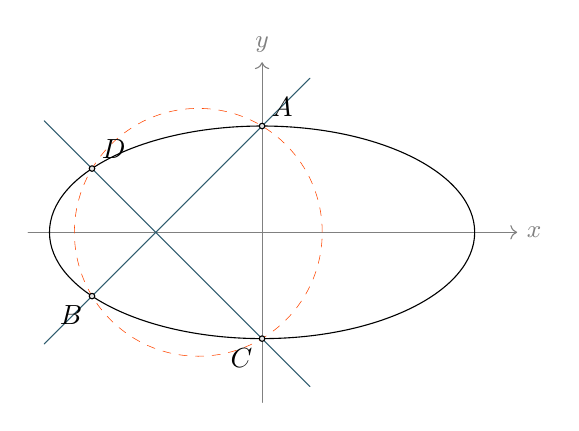
\begin{tikzpicture}[scale=1.35]
\tkzDefPoints{0/1/A,-1.6/-.6/B,0/-1/C,-1.6/.6/D,-.6/0/O}
\draw[->,gray] (-2.2,0)--(2.4,0) node[right]{$x$};
\draw[->,gray] (0,-1.6)--(0,1.6) node[above]{$y$};
\draw[black] (0,0) ellipse (2 and 1);
\tkzDrawCircle[dashed,color=OrangeRed](O,A)
\draw[coverfgcolor] (-2.05,-1.05)--(.45,1.45);
\draw[coverfgcolor] (-2.05,1.05)--(.45,-1.45);
\tkzDrawPoints(A,B,C,D)
\tkzLabelPoints[above right](A,D)\tkzLabelPoints[below left](B,C)
\end{tikzpicture}
\figcaption{两条弦与椭圆共有四点；从曲线系中挑出经过它们的圆。}
\end{center}
\level{核算而不是解题必需}四点恰为 $(0,1),(-8/5,-3/5),(0,-1),(-8/5,3/5)$。代入圆方程均成立。这是结果复核；曲线系证明本身没有依赖求出这些坐标。
\section{推广与它的适用边界}
椭圆 $x^2/a^2+y^2/b^2=1$，$a>b>0$，被两条非竖直直线
\[
 y=mx+p,\qquad y=-mx+q
\]
截得四个互异实点。令
\[
 F=x^2/a^2+y^2/b^2-1,
 \quad G=(y-mx-p)(y+mx-q).
\]
由于 $G$ 的 $xy$ 项抵消，$F+tG$ 的平方项系数分别为 $a^{-2}-tm^2$、$b^{-2}+t$。取
\[
 t=\frac{a^{-2}-b^{-2}}{1+m^2},\qquad
 k=\frac{a^{-2}+m^2b^{-2}}{1+m^2}>0,
\]
便得到圆型方程。该方程已含四个互异实点，所以不是虚圆或点圆，四点共圆。

\begin{keybox}{为什么不能把它当作万能技巧}
一般两条直线的乘积有 $xy$ 项。要成为圆，需要同时消掉 $xy$ 并令平方项系数相等，一个参数通常不能完成两个独立条件。曲线系也不能免除交点互异、实数性、分母非零和参数范围的检查。
\end{keybox}
\section{矩阵观点与三种退化成员\quad 选读}
一般二次式写为 $X^{\mathsf T}MX$，其中 $X=(x,y,z)^{\mathsf T}$，
\[
 M=\begin{pmatrix}A&B/2&D/2\\B/2&C&E/2\\D/2&E/2&F\end{pmatrix}.
\]
在 $z=1$ 恢复 $Ax^2+Bxy+Cy^2+Dx+Ey+F=0$。曲线束是 $X^{\mathsf T}(\lambda M_1+\mu M_2)X=0$。当矩阵行列式为零时，二次曲线在复射影意义下退化；实数范围内可能是一对实直线、共轭虚直线或重直线，不能一概画成两条实直线。

四个一般位置的点 $A,B,C,D$（任三点不共线）对应三种配对：$(AB)\cup(CD)$、$(AC)\cup(BD)$、$(AD)\cup(BC)$，它们都是经过四点的退化二次曲线。这解释了为什么把两条直线的方程相乘，经常是曲线系的自然入口。

\level{与共线共面的连接}一次方程的线性组合保留直线或平面的公共点；二次方程的线性组合保留曲线的公共点。共同的思想是“保留约束，改变对象的表达”。初中阶段把它用于圆幂、根轴，高中阶段再发展为曲线系即可。

\chapter{选读 用一个向量恒等式证明费尔巴哈定理}
\level{竞赛拓展：本章独立补证，不作为两道压轴题的先修要求}
前文说明了费尔巴哈定理的内容。这里给出一条可逐项核对的向量证明，同时处理内切圆和三个旁切圆。它需要有向面积、向量平方展开和海伦公式；初次学习时可以先跳过，主线证明不依赖本章。向量证明的参考见 Michael Scheer 的\href{https://arxiv.org/abs/1107.1152}{A Simple Vector Proof of Feuerbach's Theorem}；以下把内外切圆统一在一个带符号的计算中。

\section{两条准备公式}
首先，海伦公式与外接半径面积式为
\[
 \Delta^2=s(s-a)(s-b)(s-c),\qquad abc=4R\Delta.
\]
为免把它们作为无来历的额外工具，前式可由余弦定理和 $2\Delta=bc\sin A$ 推得：
\[
 16\Delta^2=4b^2c^2-(b^2+c^2-a^2)^2
 =(a+b+c)(-a+b+c)(a-b+c)(a+b-c).
\]
后式则由 $a=2R\sin A$ 与面积式直接相乘得到。

其次，若点 $X$ 写成仿射组合
\[
 X=\alpha A+\beta B+\gamma C,\qquad \alpha+\beta+\gamma=1,
\]
则对任意点 $Y$ 有
\begin{equation}\label{eq:weighted-distance-feuerbach}
 XY^2=\alpha AY^2+\beta BY^2+\gamma CY^2
 -\beta\gamma a^2-\gamma\alpha b^2-\alpha\beta c^2.
\end{equation}
\begin{proof}
以 $Y$ 为原点，把 $|\alpha\mathbf a+\beta\mathbf b+\gamma\mathbf c|^2$ 展开，再用
$2\mathbf a\cdot\mathbf b=|\mathbf a|^2+|\mathbf b|^2-c^2$ 等式替换交叉项，平方项系数由 $\alpha+\beta+\gamma=1$ 化成所需形式。该恒等式不要求系数都为正。
\end{proof}
三个系数也等于有向面积比
\[
 \alpha=\frac{[XBC]}{[ABC]},\qquad
 \beta=\frac{[AXC]}{[ABC]},\qquad
 \gamma=\frac{[ABX]}{[ABC]}.
\]
这可由三角形有向面积的行列式展开验证。因而令 $t=s-a$，由到三边距离相等及 $\Delta=rs=r_At$，有
\[
 I=\frac{aA+bB+cC}{2s},\qquad
 I_A=\frac{-aA+bB+cC}{2t}.
\]
$I_A$ 在 $BC$ 的另一侧，故第一个有向面积比为负；这正是唯一改变的符号。

\section{先算九点圆心到三个顶点的距离}
仍以 $O$ 为原点，使用前文已经证明的
$\mathbf h=\mathbf a+\mathbf b+\mathbf c$、$\mathbf n=\mathbf h/2$。于是
\[
 4AN^2=|\mathbf a-\mathbf b-\mathbf c|^2
 =R^2-a^2+b^2+c^2,
\]
另外两式循环得到。最后一步只需代入
$\mathbf a\cdot\mathbf b=R^2-c^2/2$。

\section{一次计算同时证明四个相切}
取 $(x,y,z)=(a,b,c)$ 或 $(-a,b,c)$，令 $q=x+y+z$，并设
\[
 X=\frac{xA+yB+zC}{q}.
\]
这两种情况分别给出 $X=I$ 和 $X=I_A$，且 $x^2=a^2,y^2=b^2,z^2=c^2$。将 $Y=N$ 代入式\eqref{eq:weighted-distance-feuerbach}，得到
\begin{align*}
 NX^2
 &=\frac{R^2}{4}
 +\frac{q(x^2+y^2+z^2)-2(x^3+y^3+z^3)}{4q}
 -\frac{xyz}{q}\\
 &=\frac{R^2}{4}
 +\frac{(-x+y+z)(x-y+z)(x+y-z)}{4q}
 -\frac{xyz}{2q}.
\end{align*}
其中第二行只是三次多项式展开与合并。第一行最后一项使用
$yz\,a^2+zx\,b^2+xy\,c^2=xyz(x+y+z)$。

当 $(x,y,z)=(a,b,c)$ 时，$q=2s$。上式结合海伦公式、$abc=4R\Delta$，化为
\[
 NI^2=\frac{R^2}{4}
 +\frac{(s-a)(s-b)(s-c)}{s}-\frac{abc}{4s}
 =\frac{R^2}{4}+r^2-Rr
 =\left(\frac R2-r\right)^2.
\]
非等边情形由欧拉不等式的等号条件得 $R/2>r$，故 $NI=R/2-r>0$，两圆圆心距等于半径差，九点圆与内切圆内切。

当 $(x,y,z)=(-a,b,c)$ 时，$q=2t$，三因子的乘积为 $8s(s-b)(s-c)$，而 $xyz=-abc$。于是
\[
 NI_A^2=\frac{R^2}{4}
 +\frac{s(s-b)(s-c)}{t}+\frac{abc}{4t}
 =\frac{R^2}{4}+r_A^2+Rr_A
 =\left(\frac R2+r_A\right)^2.
\]
圆心距等于半径和，故九点圆与 $A$ 旁切圆外切。循环换字母得到其余两旁切圆的外切结论。这就完成了费尔巴哈定理的证明。等边情形则 $NI=0$、$r=R/2$，两圆重合，应与单切点相切区分。

\chapter{小练习 把判定条件落实到纸面}
\level{由浅入深，先独立写出所用判定，再看提示}
\begin{enumerate}
\item $D,E$ 分别是 $\triangle ABC$ 中从 $B,C$ 向 $AC,AB$ 作高的垂足。证明 $B,C,D,E$ 共圆，并写出圆心。
\item $\triangle ABC$ 中，$D,E$ 分别为 $BC,CA$ 的中点，直线 $DE$ 与 $AB$ 平行。解释为什么此时不能再令 $F=DE\cap AB$ 后套梅涅劳斯。
\item $\triangle ABC$ 的 $BC,CA$ 上取 $D,E$，使 $BD:DC=2:1$、$CE:EA=3:1$。若 $DE$ 交直线 $AB$ 于 $F$，求 $AF:FB$，并判断 $F$ 的位置。
\item 非等边三角形中 $OH=12$，求 $OG,GH,ON$。再说明仅有 $R=5$ 时，能否确定 $r$。
\item 已知三角形 $R=5,r=2$，求 $OI$。若又有 $O=I$，原数值是否可能？
\item $M$ 为外接圆不含 $A$ 的弧 $BC$ 中点，$MB=3$、$AI=8$。求 $MI$ 和 $Rr$。
\item 两个非同心圆的三个等幂点 $X,Y,Z$ 为何共线？若把条件改为“分别对三个不同圆等幂”，为什么表述不够明确？
\item 空间中 $A=(0,0,0),B=(2,0,0),C=(0,3,0),D=(1,1,t)$。求使四点共面的 $t$，并把结论写成向量二项表示。
\end{enumerate}

\section{参考解答}
\begin{enumerate}
\item $\angle BDC=\angle BEC=90^\circ$，两点都在以 $BC$ 为直径的圆上，圆心为 $BC$ 中点。若原三角形直角造成点重合，应把题目理解为对应的非退化情形。
\item 因两线平行，没有有限交点 $F$；不能为了套定理凭空引入一个不存在的点。应直接用中位线定理。
\item 梅涅劳斯有向比给出 $6\,\overline{AF}/\overline{FB}=-1$，故普通长度 $AF:FB=1:6$。$D,E$ 都内分，因此 $F$ 外分；$AF<FB$，故在 $BA$ 方向越过 $A$ 的延长线上。
\item $OG=4,GH=8,ON=6$。仅知 $R$ 不能确定 $r$；固定外接圆上可取形状不同的三角形。
\item $OI=\sqrt{5(5-4)}=\sqrt5$。若 $O=I$ 则 $R=2r$，与 $5\ne4$ 矛盾。
\item $MI=MB=3$，且 $AI\cdot IM=2Rr$，所以 $Rr=12$。
\item 三点都在\emph{同一对圆}的根轴上。若“等幂”所比较的圆对随点改变，就不能保证它们属于同一条根轴。
\item 行列式为 $6t$，故 $t=0$；此时 $\overrightarrow{AD}=\tfrac12\overrightarrow{AB}+\tfrac13\overrightarrow{AC}$。
\end{enumerate}

\backmatter
\chapter{资料与继续学习}
下面的来源用于核对定理的适用条件和延伸阅读，正文证明均重新组织。检索日期为 2026 年 11 月 15 日。网络资料不替代用户提供的试题原件。
\begin{enumerate}
\item \href{https://users.math.uoc.gr/~pamfilos/Yiu.pdf}{Paul Yiu，Introduction to the Geometry of the Triangle，系统三角形几何讲义}。
\item \href{https://mathcircle.berkeley.edu/sites/default/files/archivedocs/2014_2015/lectures/1415lecturespdf/Int\%20II\%20-\%202015.01.20.pdf}{Berkeley Math Circle，Triangle Centers，弧中点与内旁心}。
\item \href{https://metric.ma.ic.ac.uk/metric_public/vectors/vector_coordinate_geometry/scalar_triple_product.html}{Imperial College，Scalar Triple Product，混合积与共面}。
\item \href{https://gkfweb.math.illinois.edu/oldnew/math403/public/dilatations/dilatations.html}{University of Illinois，Dilatations，欧拉线与九点圆}。
\item \href{https://sites.math.washington.edu/~king/coursedir/m444a04/class/class29.html}{University of Washington，Excentral Triangle，旁心三角形}。
\item \href{https://mathworld.wolfram.com/MenelausTheorem.html}{Wolfram MathWorld，Menelaus Theorem，梅涅劳斯定理}。
\item \href{https://mathworld.wolfram.com/CevasTheorem.html}{Wolfram MathWorld，Ceva's Theorem，塞瓦定理}。
\item \href{https://mathworld.wolfram.com/RadicalLine.html}{Wolfram MathWorld，Circle Power 与 Radical Line，圆幂与根轴}。
\item \href{https://mathworld.wolfram.com/SimsonLine.html}{Wolfram MathWorld，Simson Line 与 Miquel's Theorem，垂足共线和米克尔点}。
\item \href{https://arxiv.org/abs/1107.1152}{Michael Scheer，A Simple Vector Proof of Feuerbach's Theorem，2011}。
\item \href{https://www.geometrie.tuwien.ac.at/geom/ig/peternell/peternell_odehnal_rev2.pdf}{M. Peternell 与 B. Odehnal，Convolution surfaces of quadratic triangular Bézier surfaces，第 4.2 节曲线束}。
\item \href{https://www.cs.utexas.edu/~EWD/ewd10xx/EWD1017.PDF}{E. W. Dijkstra，Fillers at a YoP-institute 中的 Pompeiu 定理证明}。
\item \href{https://ctan.org/pkg/tkz-euclide}{Alain Matthes，tkz-euclide 官方手册，图形命令的依据}。
\end{enumerate}
\end{document}
